% Apêndice: telas da aplicação web (capturas do protótipo em funcionamento).
% As imagens estão em figuras/telas/. Os dados exibidos são do protótipo real;
% \pendente marca as capturas que devem ser refeitas depois da remontagem do sonar.

\section{Telas da aplicação}\label{sec:apendice-telas}

Esta seção reúne capturas da aplicação web em funcionamento com o protótipo. A navegação
tem três áreas principais (Início, Resumo e Saúde do gato) e uma página por sensor, aberta ao
tocar em qualquer cartão, marcador da planta ou evento da linha do tempo.

\pendente{Refazer as capturas da caixa de areia depois de remontar o sonar: os números de
visitas exibidos vêm de disparos falsos do sensor montado a 17,8~cm da superfície
(ver Seção~\ref{sec:resultados}).}

\begin{figure}[htbp]
  \centering
  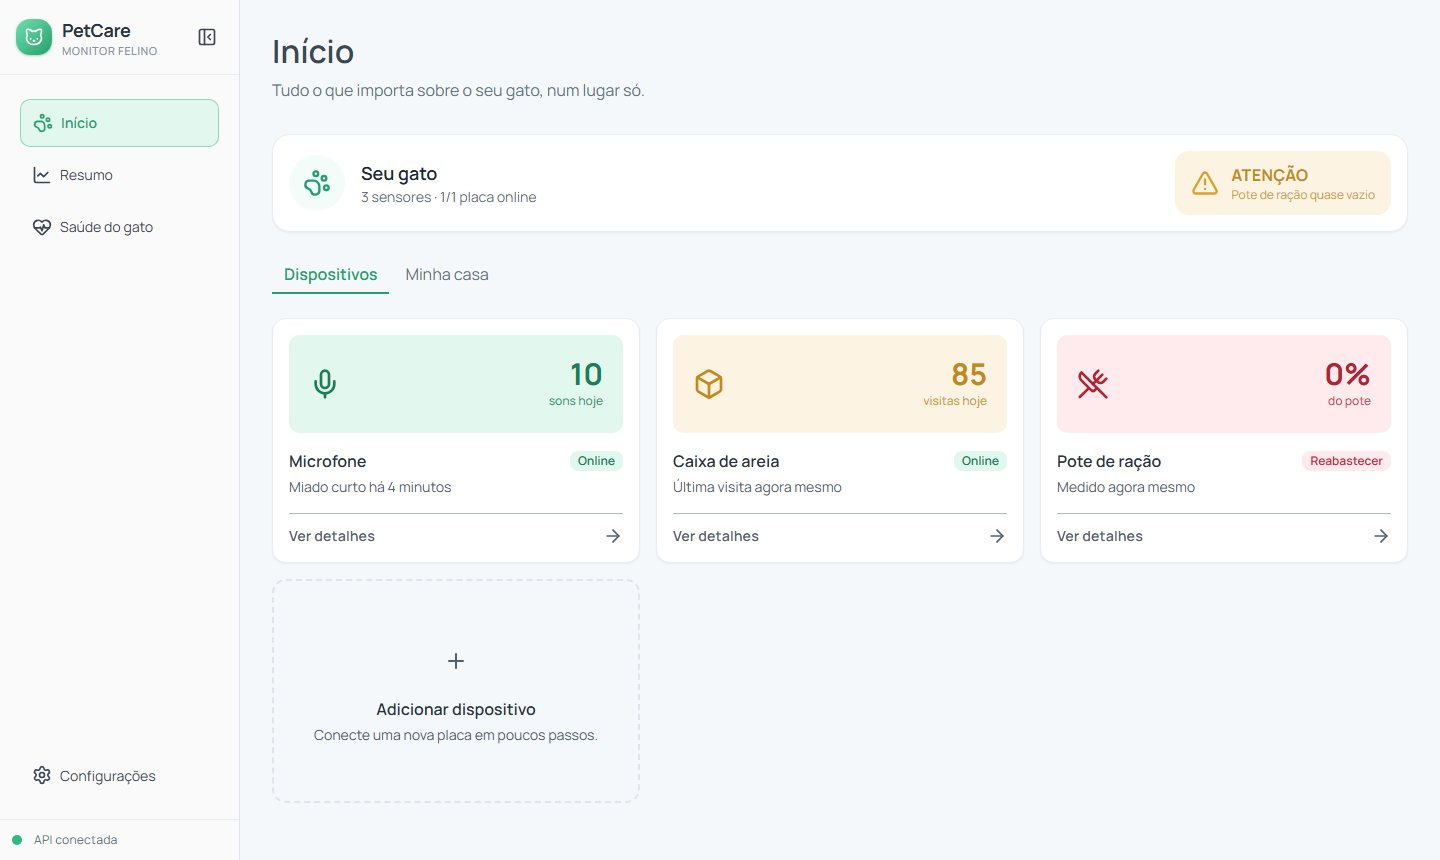
\includegraphics[width=\linewidth]{figuras/telas/inicio-dispositivos.jpg}
  \caption{Início, aba \emph{Dispositivos}: selo de estado geral da casa e um cartão por
  sensor com o valor principal do dia.}
  \label{fig:tela-inicio-dispositivos}
\end{figure}

\begin{figure}[htbp]
  \centering
  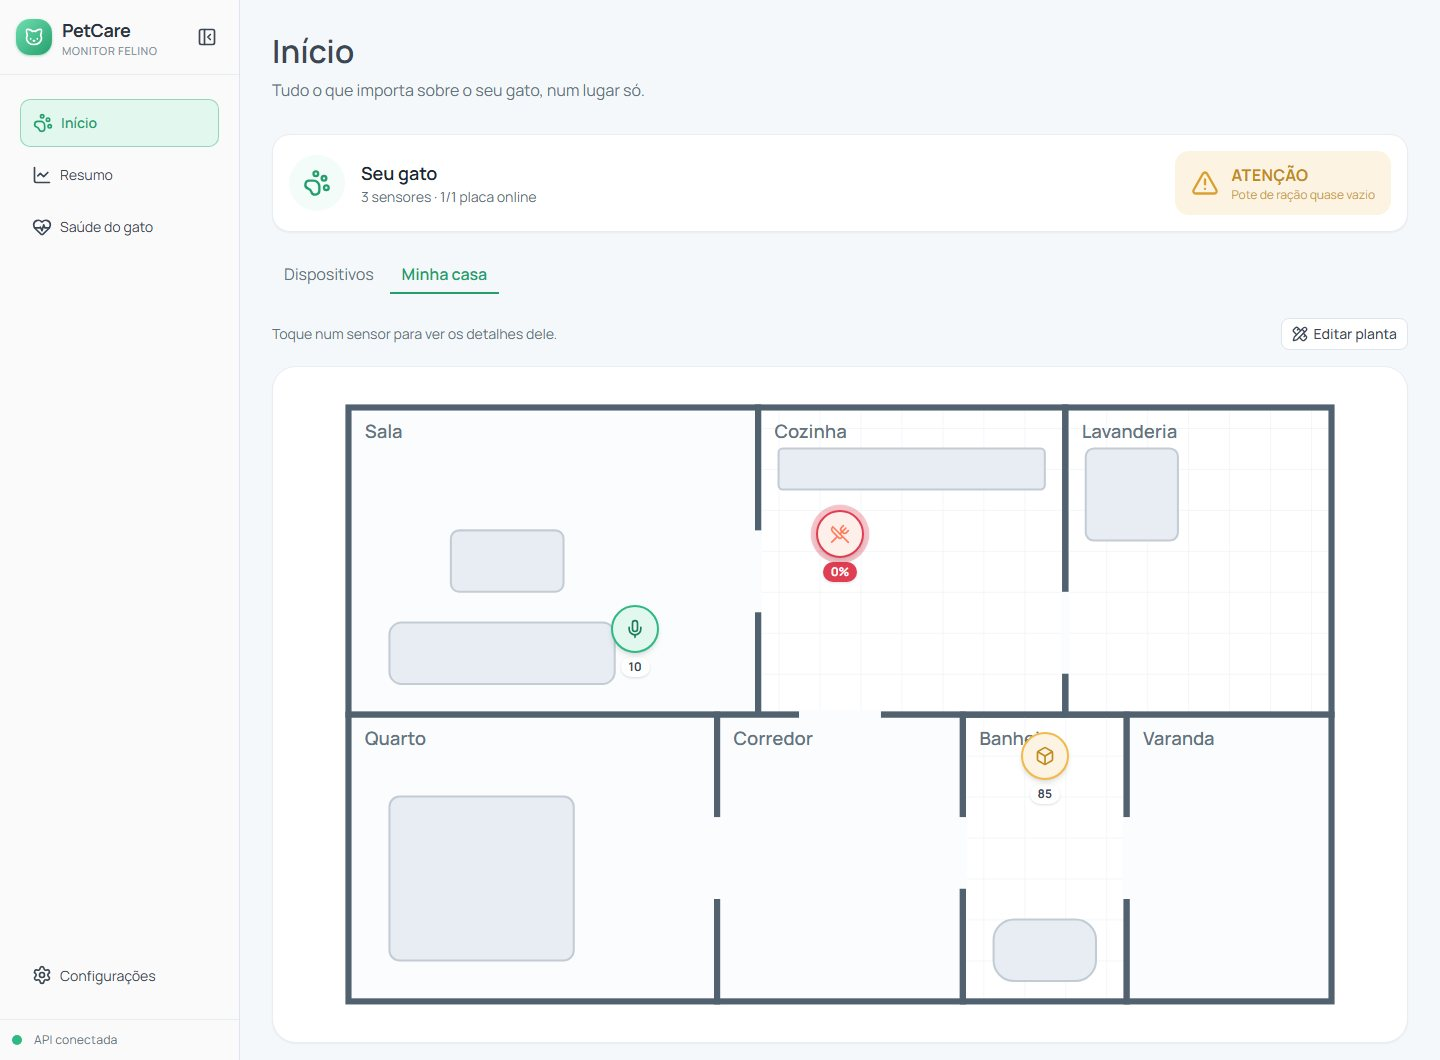
\includegraphics[width=\linewidth]{figuras/telas/inicio-casa.jpg}
  \caption{Início, aba \emph{Minha casa}: planta baixa com a posição de cada sensor.
  No modo de edição os sensores podem ser arrastados.}
  \label{fig:tela-inicio-casa}
\end{figure}

\begin{figure}[htbp]
  \centering
  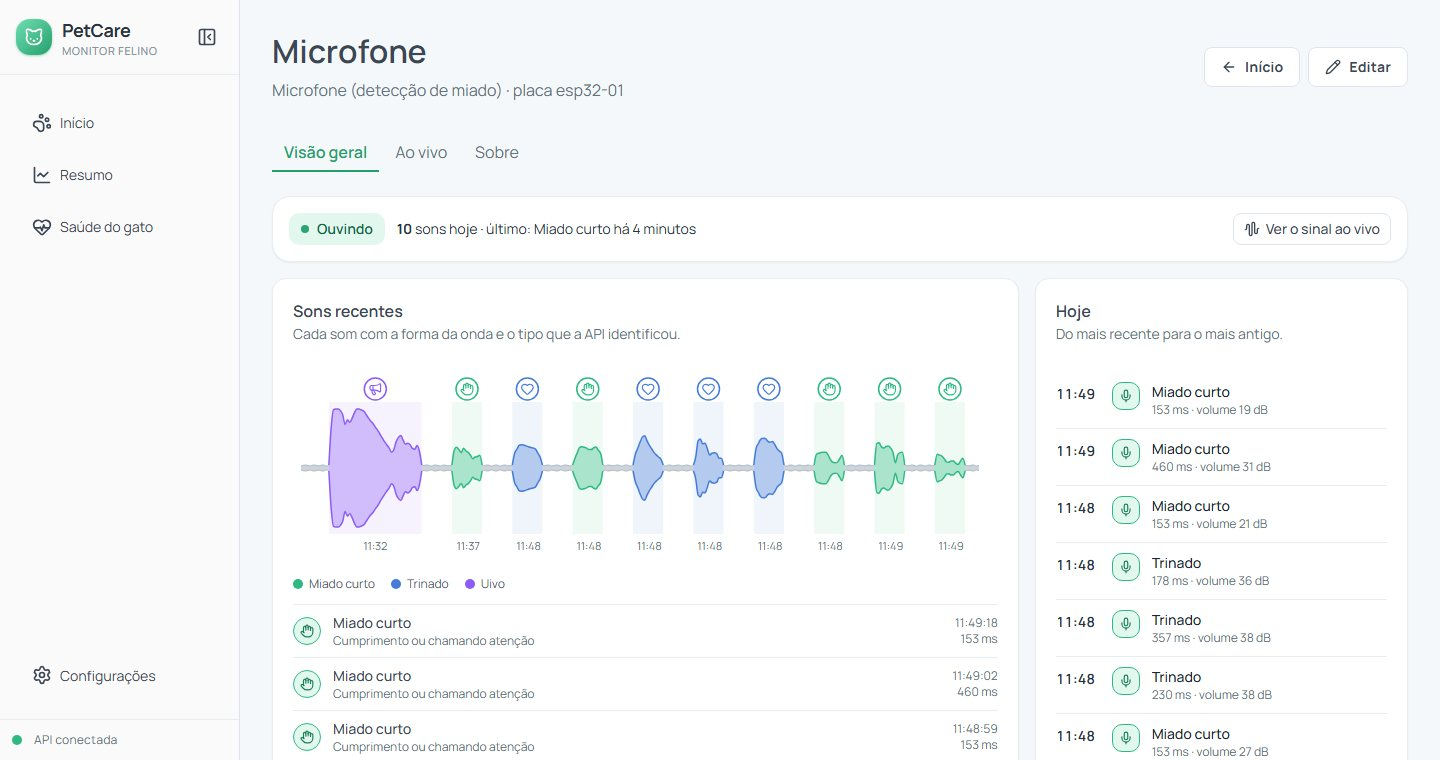
\includegraphics[width=\linewidth]{figuras/telas/sensor-microfone.jpg}
  \caption{Página do microfone, aba \emph{Visão geral}: sons recentes com a forma de onda
  (envelope de volume) e o tipo de vocalização classificado pela API.}
  \label{fig:tela-microfone}
\end{figure}

\begin{figure}[htbp]
  \centering
  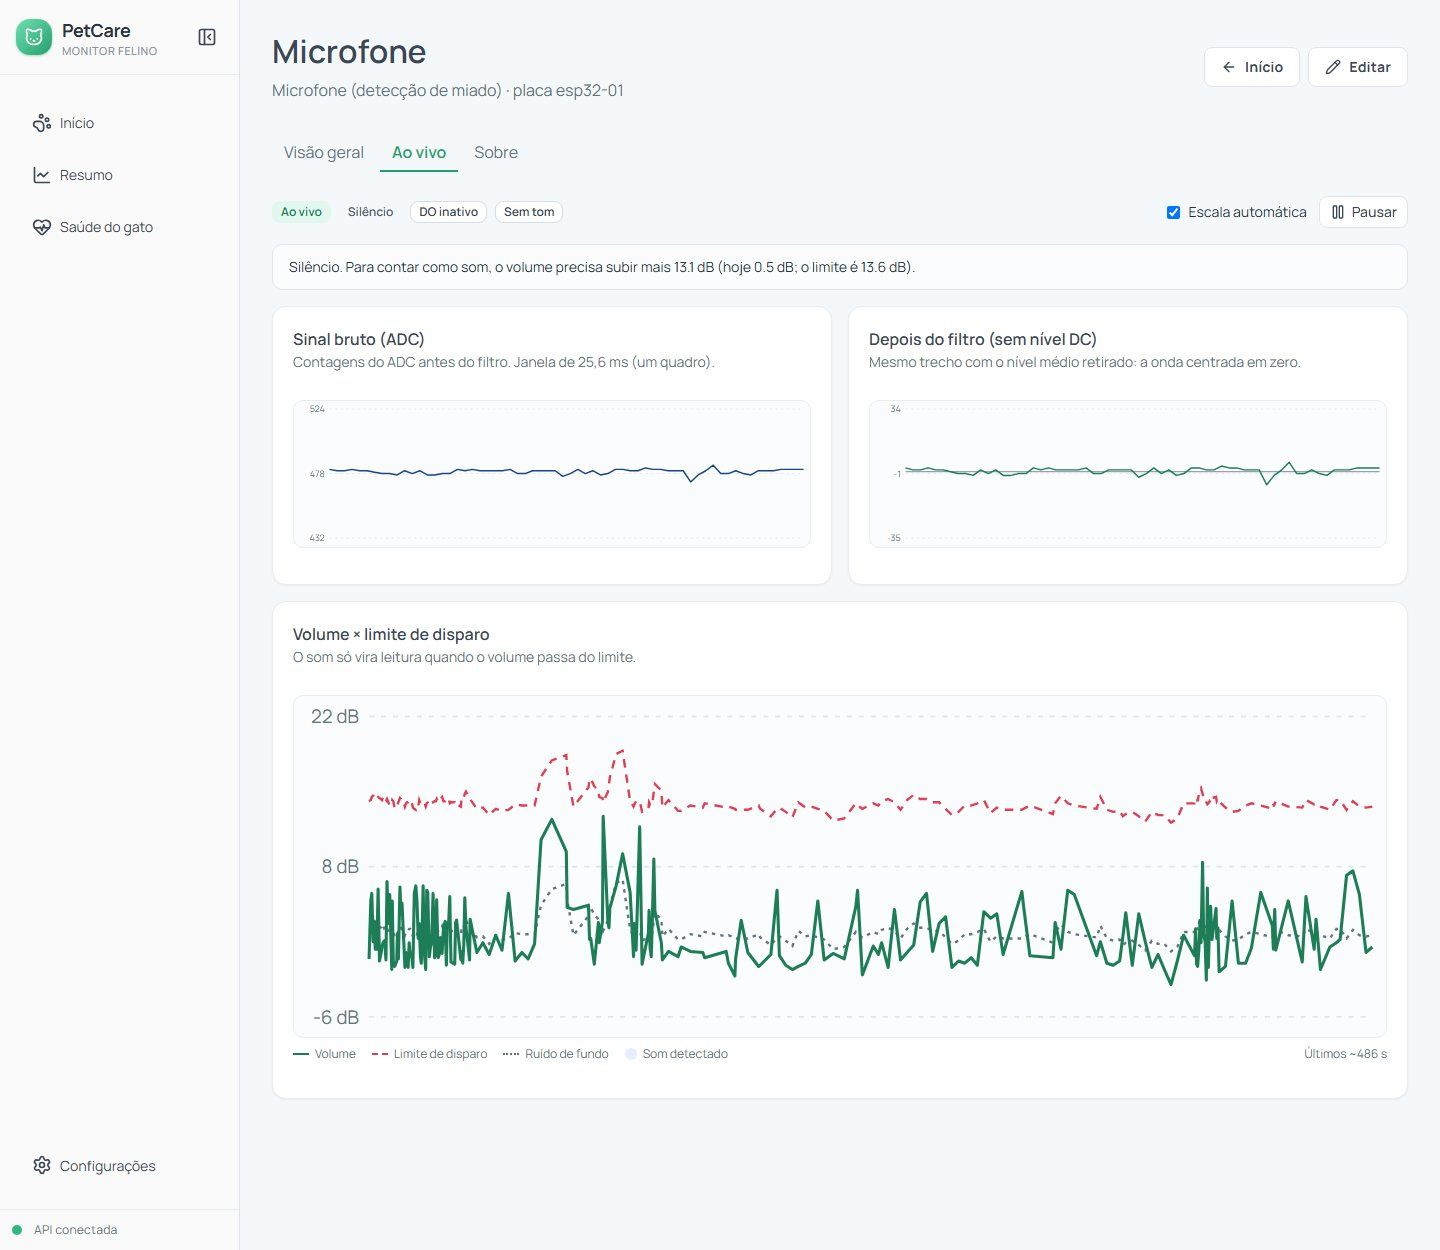
\includegraphics[width=\linewidth]{figuras/telas/sensor-microfone-ao-vivo.jpg}
  \caption{Página do microfone, aba \emph{Ao vivo}: sinal bruto do ADC, sinal após a remoção
  do nível DC e volume em relação ao limite de disparo, com diagnóstico automático.}
  \label{fig:tela-microfone-ao-vivo}
\end{figure}

\begin{figure}[htbp]
  \centering
  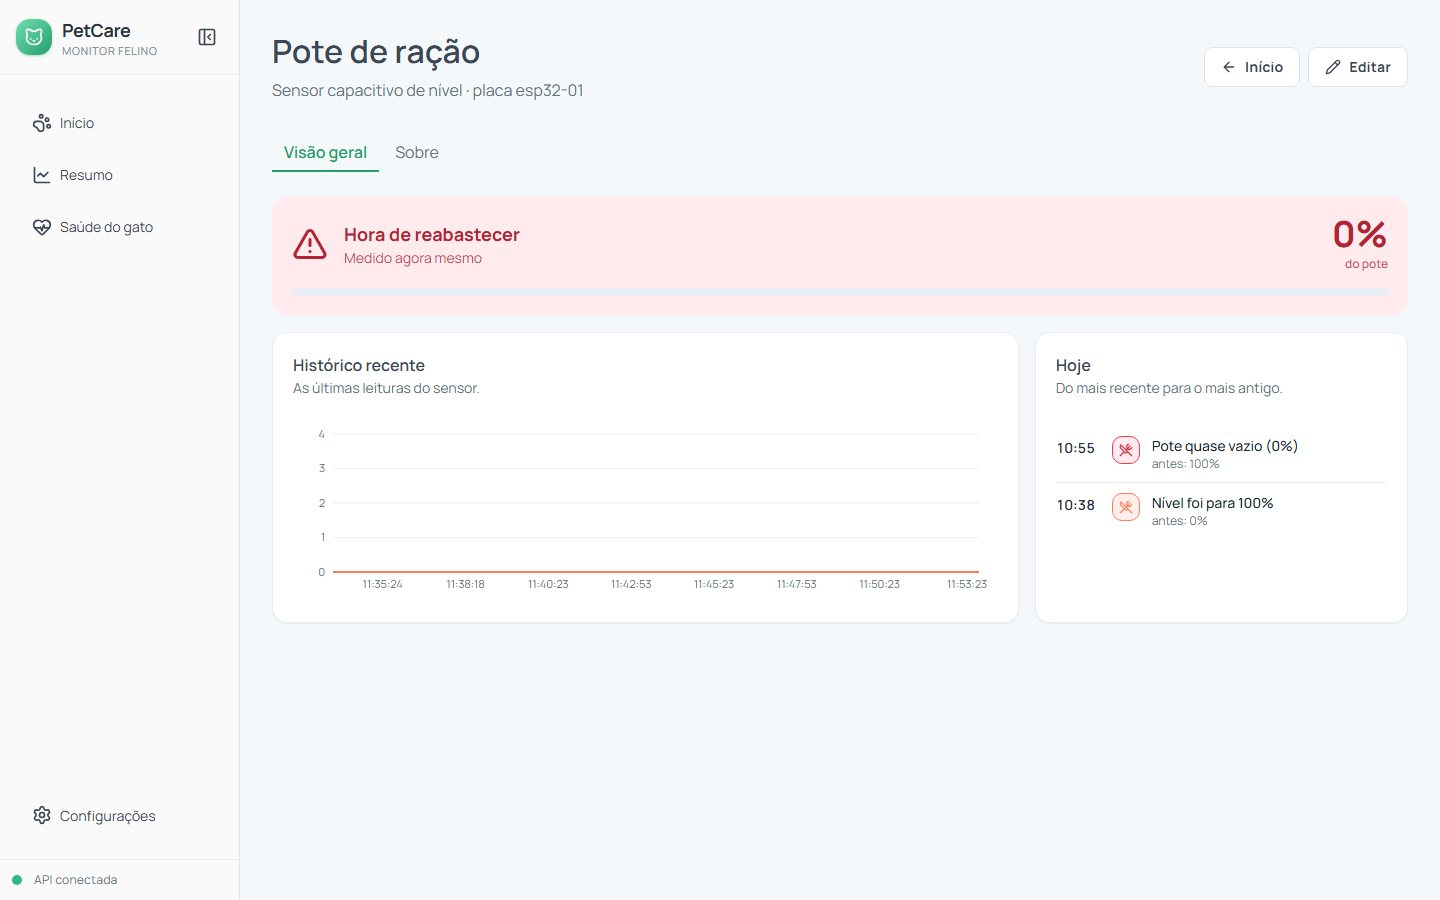
\includegraphics[width=\linewidth]{figuras/telas/sensor-pote.jpg}
  \caption{Página do pote de ração: estado atual, acontecimentos do dia e histórico das
  leituras do sensor capacitivo.}
  \label{fig:tela-pote}
\end{figure}

\begin{figure}[htbp]
  \centering
  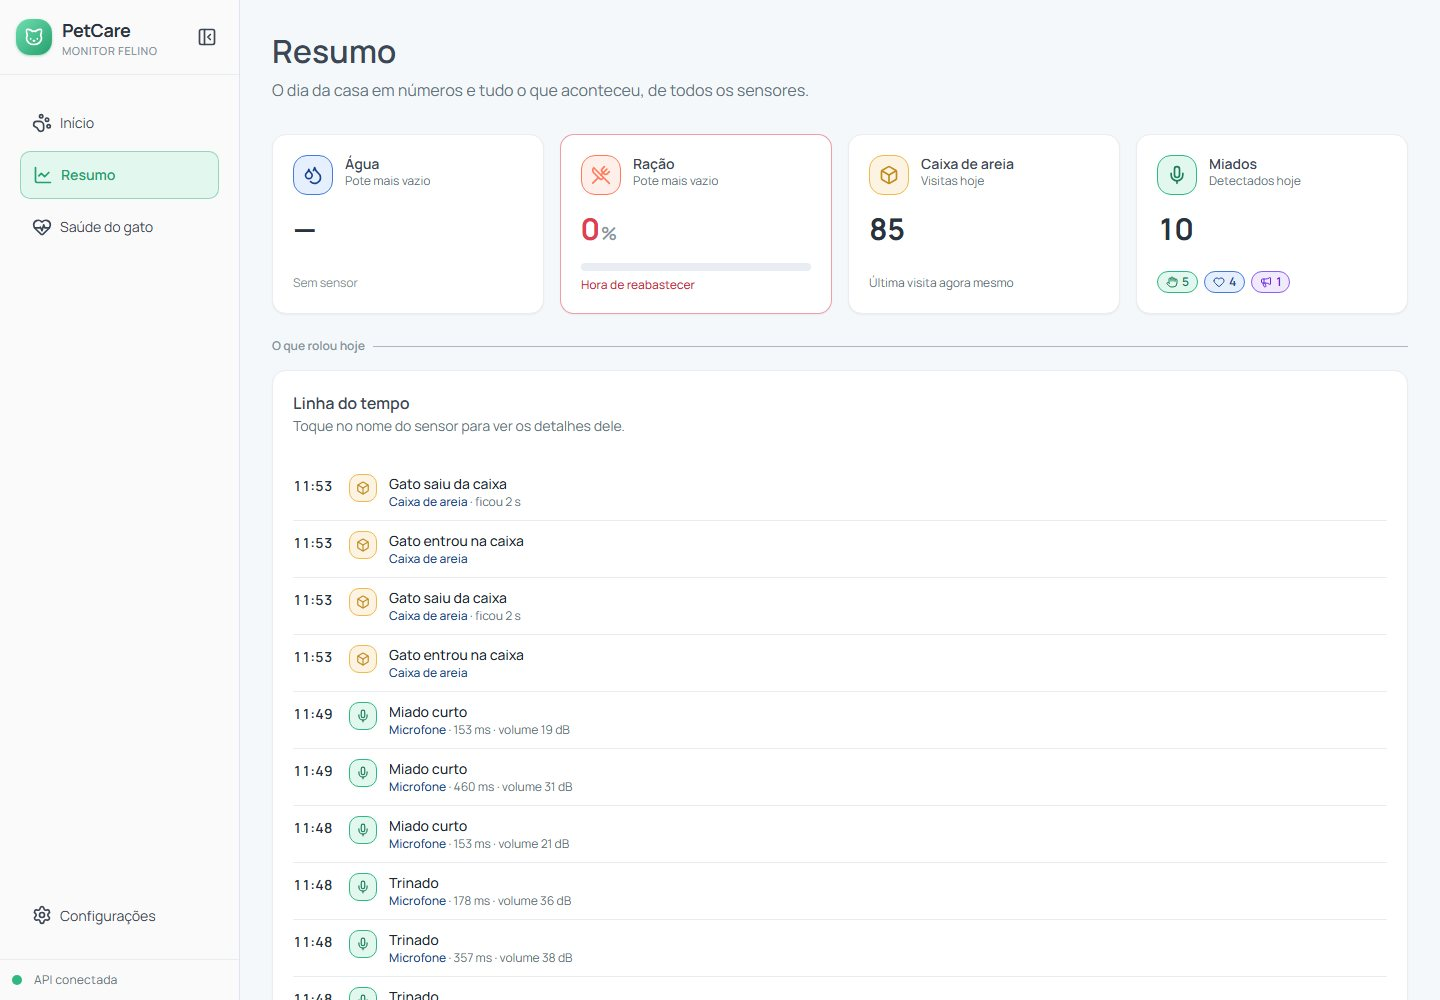
\includegraphics[width=\linewidth]{figuras/telas/resumo.jpg}
  \caption{Resumo: números do dia e linha do tempo com os acontecimentos de todos os sensores.}
  \label{fig:tela-resumo}
\end{figure}

\begin{figure}[htbp]
  \centering
  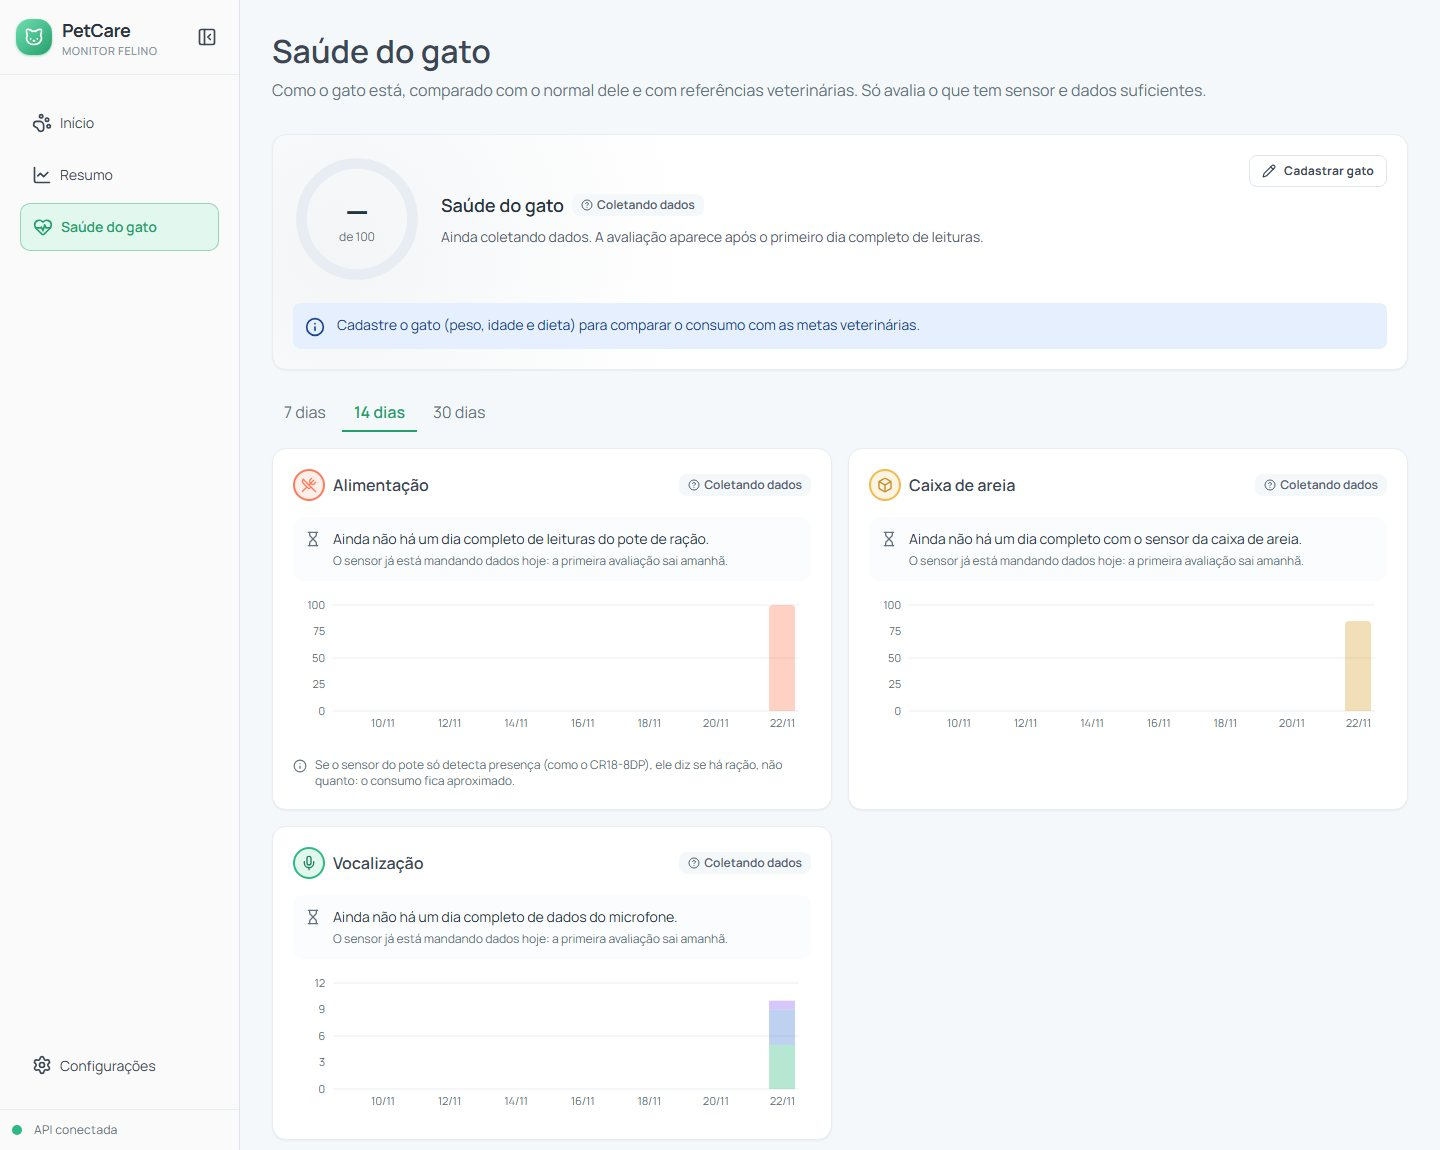
\includegraphics[width=\linewidth]{figuras/telas/saude.jpg}
  \caption{Saúde do gato: avaliação por área a partir dos dados diários. Sem dias completos
  de leitura, a aplicação indica ``Coletando dados'' em vez de um diagnóstico.}
  \label{fig:tela-saude}
\end{figure}

\begin{figure}[htbp]
  \centering
  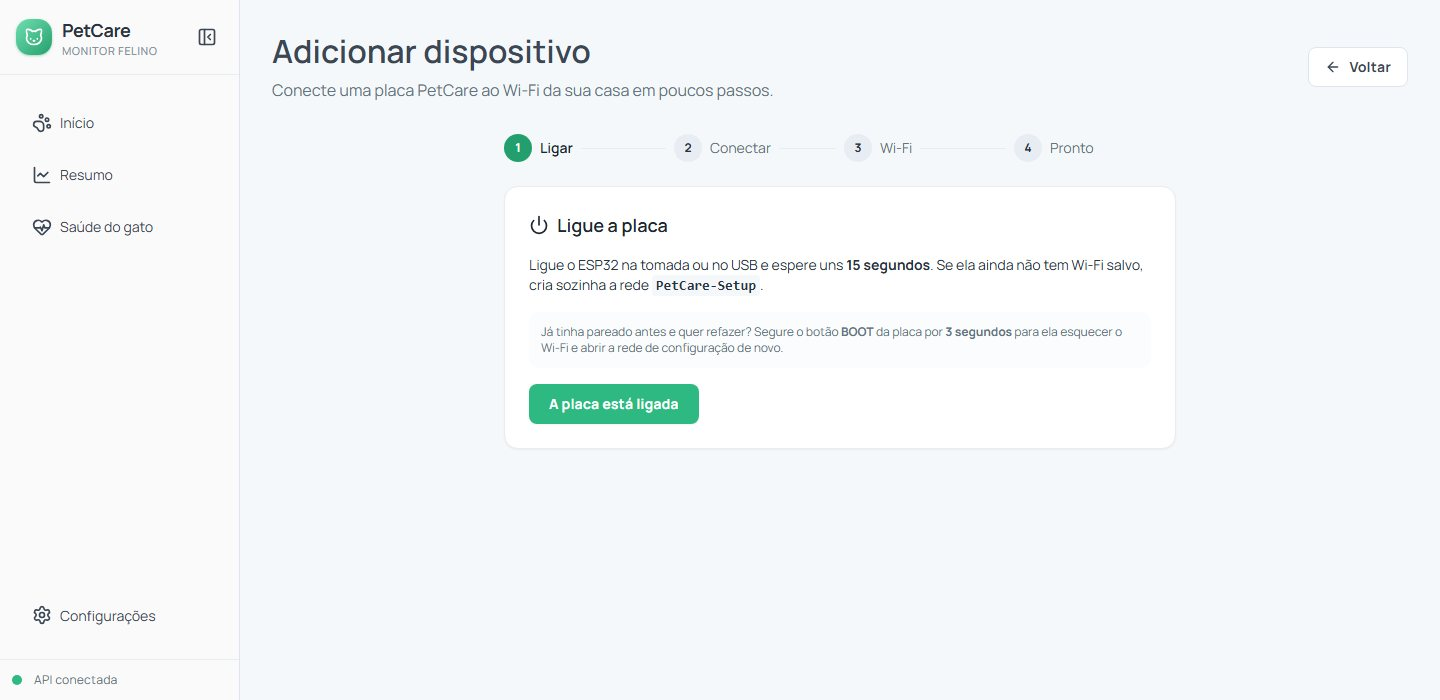
\includegraphics[width=\linewidth]{figuras/telas/adicionar-dispositivo.jpg}
  \caption{Assistente de pareamento de uma nova placa pela rede \texttt{PetCare-Setup}.}
  \label{fig:tela-adicionar}
\end{figure}
